\nomenclature[]{GPS}{Global Positioning System}
\nomenclature[]{WGS84}{World Geodetic System 1984}

\section{Generation of Waypoints}
We first address the issue of finding a discrete set of waypoints, referenced above as $R$. We chose to formulate the problem using a discrete set of waypoints, rather than deal with the case of treating the region as continuous space, since it is much easier to accurately record sensor data when the UAV has settled at a given point. Discretising the space also allows the problem to be formulated in a manner that is easier to tackle, without losing the key aspects.
%\begin{itemize}
    %\item It is more straightforward to describe the problem using a discrete set of points rather than a continuous one.
%    \item It is much easier to process sensor information if it is known exactly where this data has been captured. The UAVs may stop at each discrete waypoint to visit these locations. *Focus on this point, expand if possible*
%    \item The case of path-finding using discrete waypoints has a strong body of literature behind it
%    \item The UAVs run autopilot software which can guide them using the on-board GPS sensor
%\end{itemize}

%which are the center points of cells that partition the region of interest.
\note{set of waypoints create a voronoi partition, might be worth talking about}

\note{Above needs revision, will come back once rest of chapter has been fleshed out a bit more}
We began by assuming that the region which is to be surveyed, the \textit{region of interest}, can be described by a polygon on the x-y plane, since it allows for a discrete representation. We favour a discrete representation since it is computationally much easier to record and manipulate a set of points denoting the boundary rather than an arbitrary curve. Given this polygon, the goal is to generate a set of points, $R$, which are a uniform distance from each other in the x and y directions and lie inside the polygonal grid. These points form a regular tessellation of the region of interest. In order to do this, we employed the following methodology, using well-known algorithms:
\begin{enumerate}
    \item Find the circum-rectangle that tightly bounds the polygon, which is oriented with the x-y plane. This is shown in \ref{fig:PolygonWithBoundingRect}
    \item Generate a set of grid points in the bounding rectangle. This is shown in \ref{fig:PolygonWithBoundingRectAndGridPoints}
    \item Prune the points that lie inside the rectangle but outside the polygon. This is shown in \ref{fig:PolygonWithBoundingRectAndGridPointsPruned}
\end{enumerate}


\begin{figure}
\centering
\subfloat[Arbitrary Polygonal Region]{
  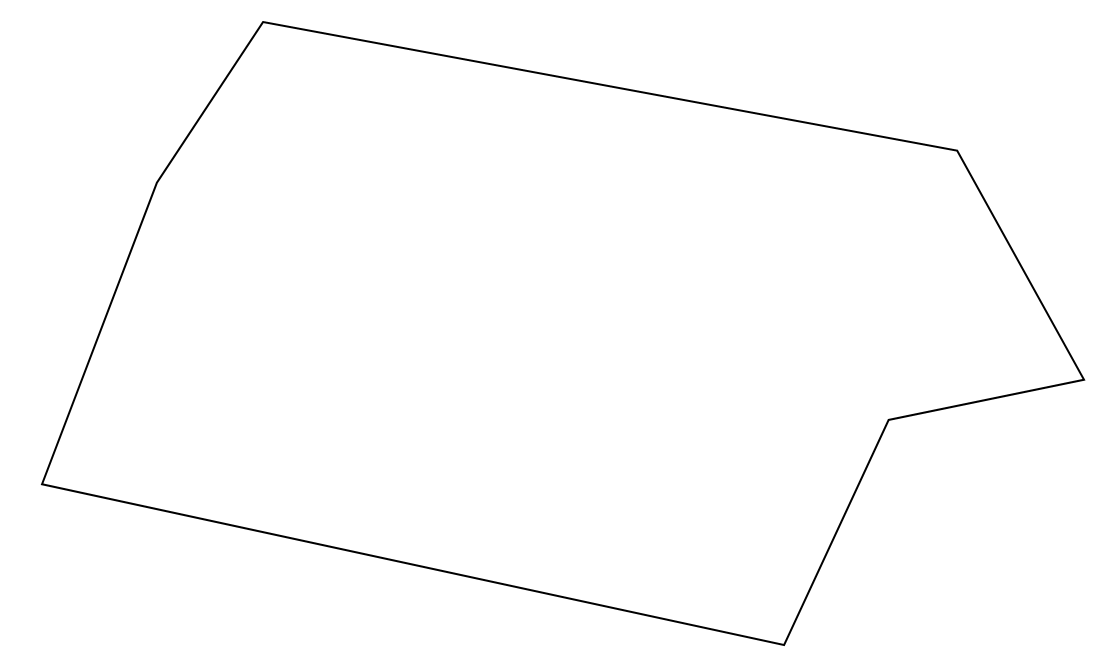
\includegraphics[width=68mm]{Chapters/MultiAgentCoverage/Figs/Polygon.PNG}\label{fig:PolygonOnly}
}
\subfloat[Bounding Rectangle Found]{
  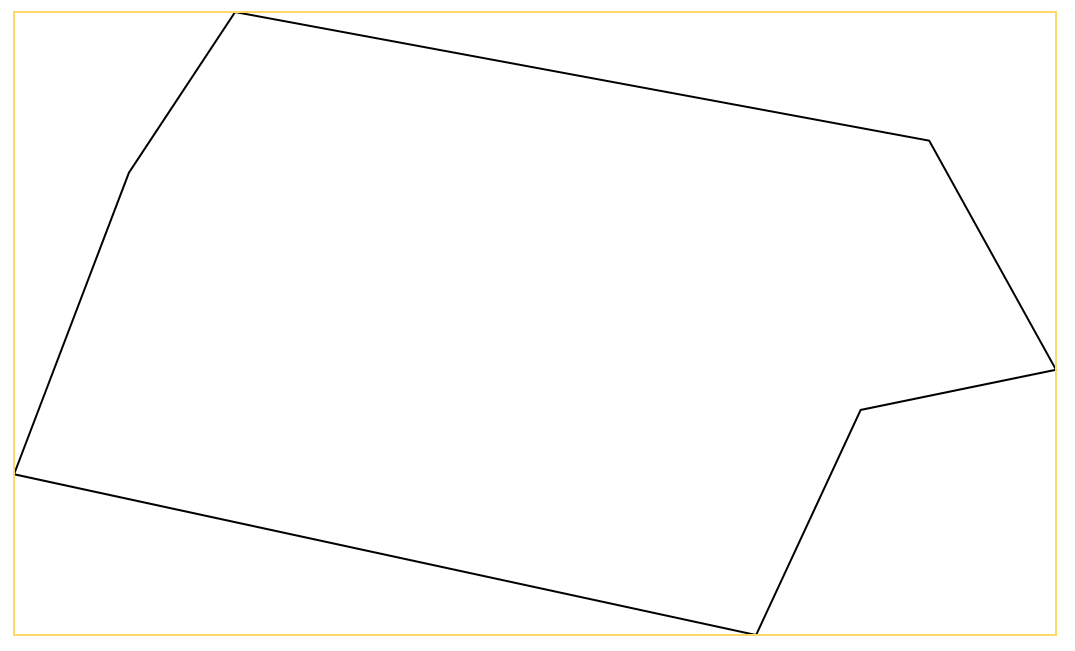
\includegraphics[width=68mm]{Chapters/MultiAgentCoverage/Figs/PolygonBoundingRect.PNG}\label{fig:PolygonWithBoundingRect}
}
\hspace{0mm}
\subfloat[Grid Points Generated in Bounding Rectangle]{
  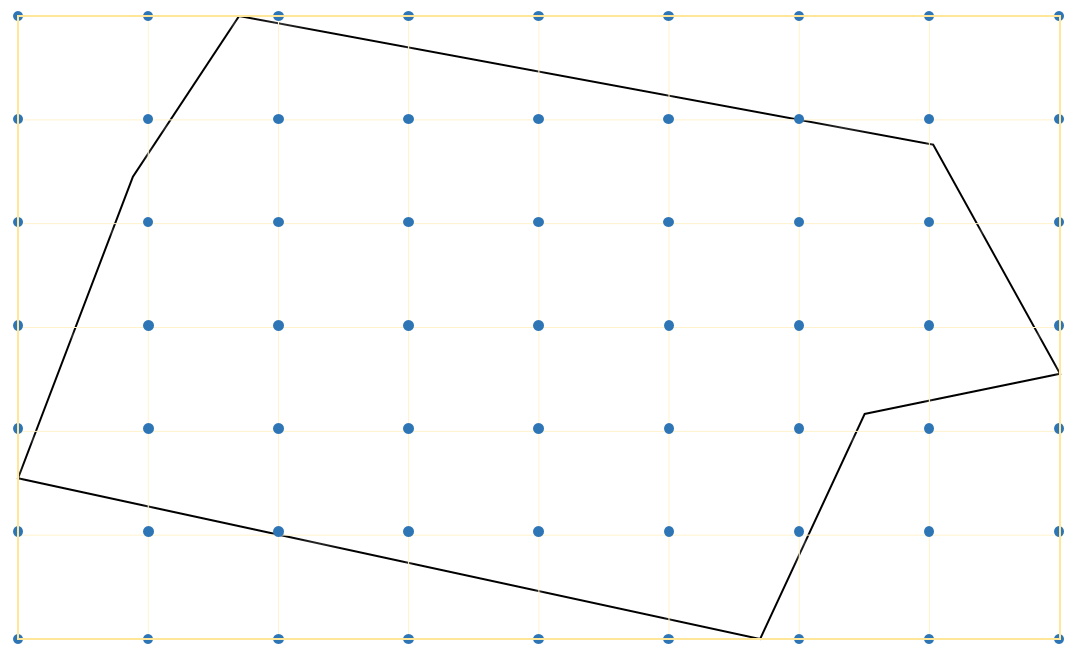
\includegraphics[width=68mm]{Chapters/MultiAgentCoverage/Figs/PolygonBoundingRectGridPoints.PNG}\label{fig:PolygonWithBoundingRectAndGridPoints}
}
\subfloat[Grid Points Outside of Polygon Pruned]{
  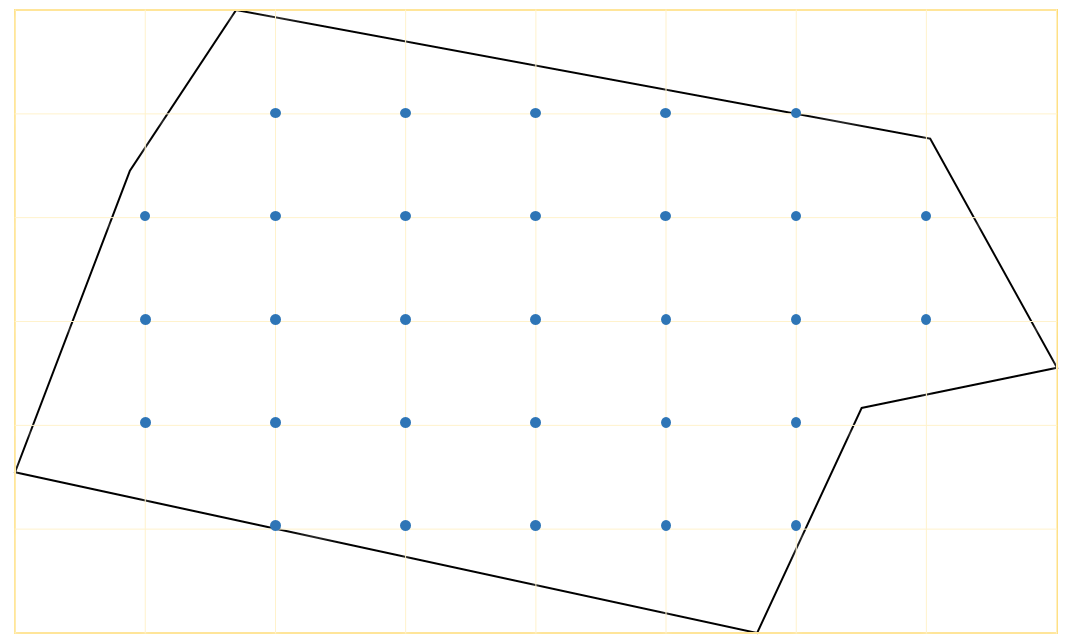
\includegraphics[width=68mm]{Chapters/MultiAgentCoverage/Figs/PolygonBoundingRectGridPointsPruned.PNG}\label{fig:PolygonWithBoundingRectAndGridPointsPruned}
}
\end{figure}

This procedure was devised with the aim of being straightforward to implement and modify. The algorithm used to carry out these steps is outlined in Algorithm \ref{alg:GridGeneration}. The algorithm is very intuitive: first, the bounding circum-rectangle is constructed from the largest and smallest x and y coordinates of the points in the polygon, outlined in lines 2-6. Then grid points in the bounding rectangle are generated in lines 7-13. Finally in lines 14-18, the grid points that lie inside the bounding rectangle but outside the polygon are pruned using the Point-in-Polygon routine which is described separately in Algorithm \ref{alg:PointInPolygon}. 


\begin{algorithm}{}
%\caption{Crossing Test for Point in Polygon based on \cite{Shimrat1962Algorithms}}
\caption{Point-in-Polygon}
\label{alg:PointInPolygon}
\begin{algorithmic}[1]
\renewcommand{\algorithmicrequire}{\textbf{Input:}}
\renewcommand{\algorithmicensure}{\textbf{Output:}}
%Input
\REQUIRE $ \newline R \quad \text{ The polygon which covers the region of interest}
%\newline R \quad \text{ The set of (x, y) points defining the polygon which covers the region of interest}
\newline P \quad \text{ A point which will be tested for containment in the polygon }
$
%Output
\ENSURE $\newline \text{True if P is contained in R else False }$

\hfill\pagebreak
\STATE polygon\_points $\leftarrow$ The set of points defining the vertices of R
\IF{x coordinate of $P$ is greater than the largest value or less than the smallest value of the x coordinates of the points in $R$}
\RETURN False
\ELSIF{y coordinate of $P$ is greater than the largest value or less than the smallest value of the y coordinates of the points in $R$}
\RETURN False


%\ELSIF{x coordinate of P is less than the smallest value of the x coordinate of all the points in R}
%\RETURN false
%\ELSIF{y coordinate of P is greater than the largest value of the y coordinate of all the points in R}
%\RETURN false
%\ELSIF{y coordinate of P is less than the smallest value of the y coordinate of all the points in R}
%\RETURN false

\ELSE
\STATE point\_in\_polygon $\leftarrow$ True
\STATE edges $\leftarrow$ the set of edges defining R
\FOR{each edge in edges}
\STATE p1 $\leftarrow$ the first point of edge
\STATE p2 $\leftarrow$ the second point of edge

\IF{(the y coordinate of $P$ lies between the  y coordinates of p1 and p2) \&
     the x coordinate of $P$ is less than the x coordinate of the point of intersection between e and the ray extended to +$\infty$ from $P$ in the +x direction}
\STATE point\_in\_polygon $\leftarrow \neg$ point\_in\_polygon
\ENDIF

\ENDFOR
\ENDIF
\end{algorithmic} 
\end{algorithm}


\begin{algorithm}{}
\caption{Algorithm to Generate a Uniformly Spaced Grid of Points in an Arbitrary Polygon}
\label{alg:GridGeneration}
\begin{algorithmic}[1]
\renewcommand{\algorithmicrequire}{\textbf{Input:}}
\renewcommand{\algorithmicensure}{\textbf{Output:}}
%Input
\REQUIRE $ \newline R \quad\text{ The set of (x, y) points defining the polygon which covers the region of interest}
\newline x\_spacing \quad\text{ The desired spacing between points in the x direction}
\newline y\_spacing \quad\text{ The desired spacing between points in the y direction}
$
%Output
\ENSURE $\newline grid\_points \quad \text{ A set of uniformly spaced (x, y) points, which define a regular } \newline \text{ tessellation of the region of interest}$

\hfill\pagebreak
\STATE waypoints $\leftarrow$ empty array

\STATE max\_x $\leftarrow$ maximum x value of all points in R
\STATE min\_x $\leftarrow$ minimum x value of all points in R
\STATE max\_y $\leftarrow$ maximum y value of all points in R
\STATE min\_y $\leftarrow$ minimum y value of all points in R

\STATE bounding\_rect $\leftarrow$ The tightest bounding rectangle which contains the polygon R defined by the points (min\_x, min\_y), (min\_x, max\_y), (max\_x, max\_y),(max\_x, min\_y).

\STATE no\_y\_points $\leftarrow \left \lfloor{\frac{max\_y - min\_y}{y\_spacing}}\right \rfloor$
\STATE no\_x\_points $\leftarrow \left \lfloor{\frac{max\_x - min\_x}{x\_spacing}}\right \rfloor$

\FOR{y\_spacing\_index = 0 to no\_y\_points}
\FOR{x\_spacing\_index = 0 to no\_x\_points}
\STATE Add the point (min\_x + x\_spacing * x\_spacing\_index, min\_y + y\_spacing * y\_spacing\_index) to grid\_points
\ENDFOR
\ENDFOR
\FOR{point in waypoints}
\IF{Point-in-Polygon(R, point) is false}
\STATE Remove point from grid\_points
\ENDIF
\ENDFOR
\RETURN waypoints
\end{algorithmic} 
\end{algorithm}

%\begin{wrapfigure}{r}{0.5\textwidth}
%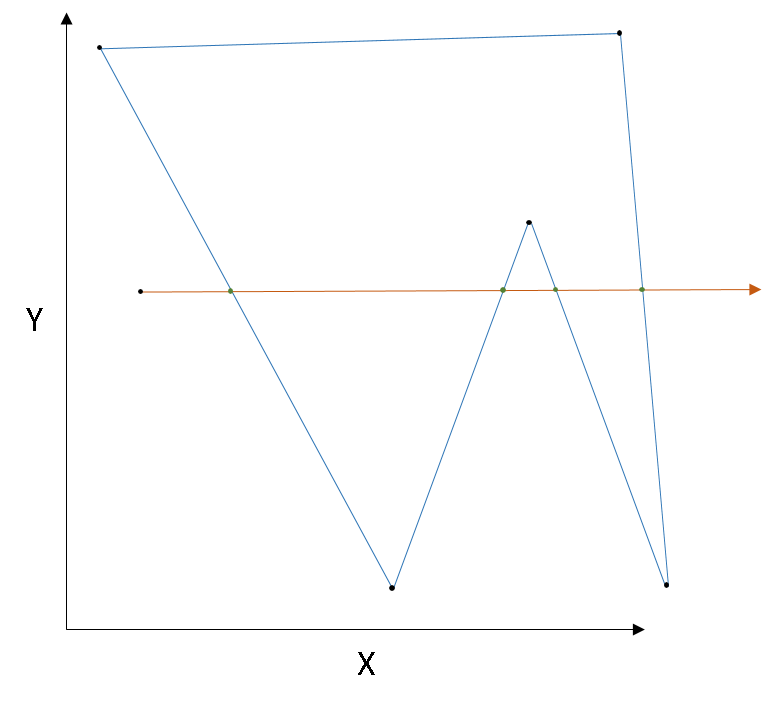
\includegraphics[width=65mm]{Chapters/MultiAgentCoverage/Figs/PointOutsidePolygon.PNG}\caption{Ray extended from point outside polygon intersects an even number of times}\label{fig:PointOutsidePolygon}
%\end{wrapfigure}

%\begin{wrapfigure}{r}{0.5\textwidth}
%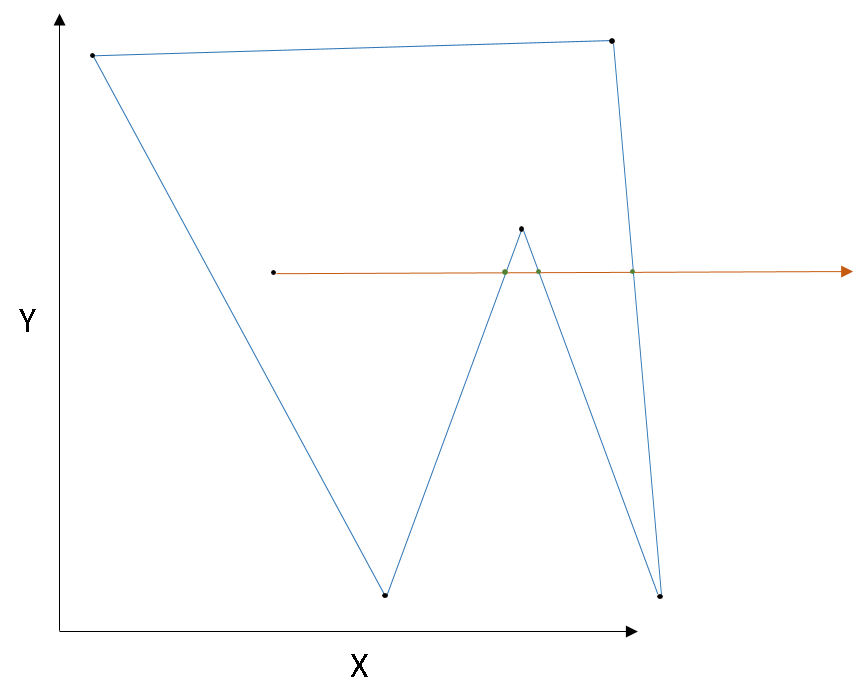
\includegraphics[width=65mm]{Chapters/MultiAgentCoverage/Figs/PointInsidePolygon.PNG}\caption{Ray extended from point inside polygon intersects an odd number of times}\label{fig:PointInsidePolygon}
%\end{wrapfigure}

We chose to use the well-known \textit{crossing test} \cite{Shimrat1962Algorithms}, which extends a ray from the point to be tested in the positive x-direction. If it crosses the boundary of the polygon an odd number of times, then it must be contained within it, otherwise it must lie outside it. This is illustrated in figures \ref{fig:PointOutsidePolygon} and \ref{fig:PointInsidePolygon}. The running time of this algorithm is dictated by the number of edges the polygon has and the size of the polygon relative to the desired tessellation spacing in the x and y directions. We did not make any optimizations other than the one outlined in lines 2-5 of Algorithm \ref{alg:PointInPolygon}, which checks whether the test point lies outside the largest and smallest x and y coordinates. but there is room to improve the running time significantly if one is dealing with particularly large regions of interest or a relatively small spacing between grid points.


\begin{figure}{}
\subfloat[Ray extended from point outside polygon intersects an even number of times]{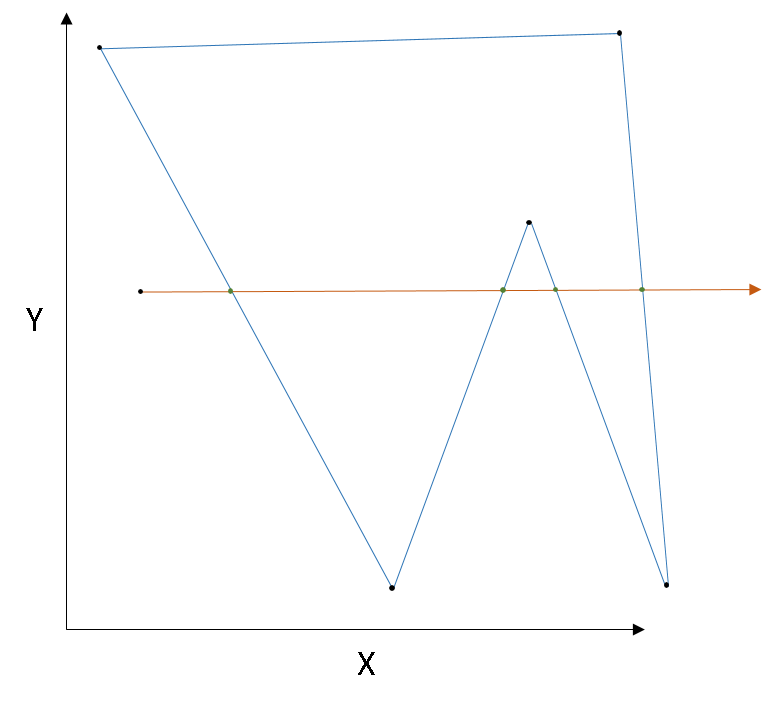
\includegraphics[width=60mm]{Chapters/MultiAgentCoverage/Figs/PointOutsidePolygon.PNG}\label{fig:PointOutsidePolygon}}
%\end{wrapfigure}
\hspace{1em}
\subfloat[Ray extended from point inside polygon intersects an odd number of times]{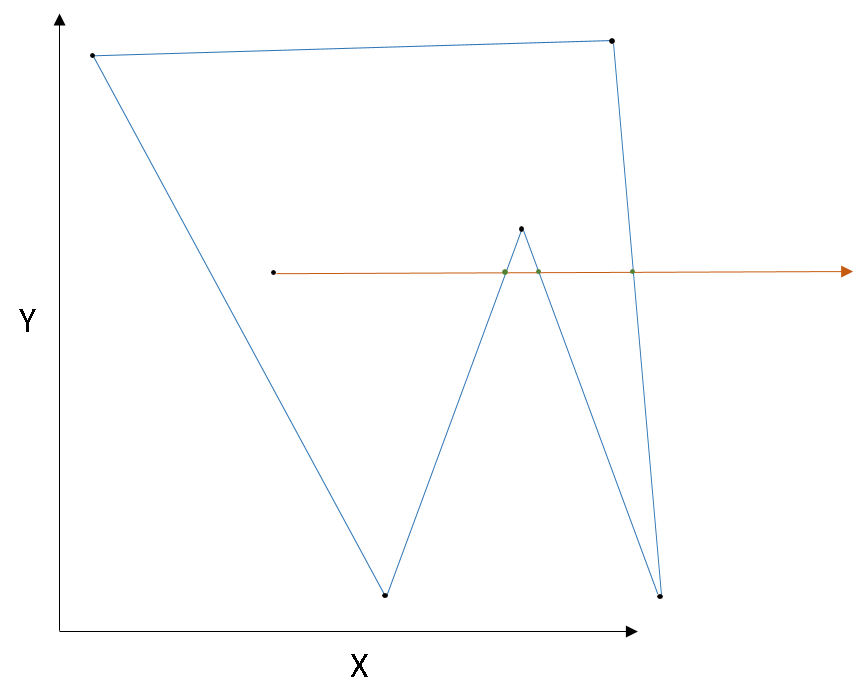
\includegraphics[width=60mm]{Chapters/MultiAgentCoverage/Figs/PointInsidePolygon.PNG}\label{fig:PointInsidePolygon}}
\end{figure}


%From a practical perspective, the region specified is defined over the earth's surface, which is not planar. For small regions, it can be assumed that this region is planar, since at 

%The generation of grid points takes this into account. The earth can be well described mathematically as an ellipsoid talk about WGS84



\subsection{Generating Waypoints as GPS Locations}
For the sake of real-world usage, it is necessary to refer to these points using some kind of reference coordinate system that UAVs can use. We provide a brief overview of how we accomplished this, without delving too far into Geographic Coordinate Systems (GCS). Since GPS is by far the most commonly system that UAVs use for navigation, we chose to design an implementation based on the \textit{World Geodetic System 1984} (WGS84) coordinate system, which is the coordinate system that GPS relies upon. The WGS84 system was created by the US department of defence and is officially documented in the official government report entitled "Department of Defense World Geodetic System 1984 Its Definition and Relationships With Local Geodetic Systems". It assumes that the datum surface is an oblate spheroid.
%, and the coordinate system uses Greenwich as the starting point. 
Coordinates are referenced using latitude, longitude and altitude, where longitude measurements range between [-180$^{\circ}$, 180$^{\circ}$], latitude measurements range between [-90$^{\circ}$, 90$^{\circ}$] and altitude measurements come in the form of meters above sea level. Greenwich is used as the \textit{prime meridian} for longitude, meaning Greenwich defines 0$^{\circ}$ longitude. The equator is used to define 0$^{\circ}$ latitude. In order to generate a grid of points in a bounding polygon as coordinates that can be referenced by the UAVs' GPS sensors, we had to make some modifications to the grid point generation algorithm outlined above. The main issue that arises is that the grid point generation algorithm assumes that the Cartesian coordinate system is used, which is obviously not valid when assuming coordinates lie on a  non-planar surface (the earth). We could simply treat the WGS84 coordinates that make the bounding polygon defining the region of interest as a plane and continue using the unmodified Algorithm \ref{alg:GridGeneration}, but for the sake of guaranteed accuracy we decided to make the following minor changes to the algorithm for use with WGS84 coordinates:
\begin{enumerate}
    \item When calculating distances, the well-known \textit{inverse solution} to finding geodesics (shortest paths along the earth's surface) is used. We also use the \textit{direct solution} to find a destination given a start point, bearing and distance. These algorithms are due to \citeauthor{Vincenty1975DirectEquations} and they take into account the non-planar nature of the WGS84 coordinate system \cite{Vincenty1975DirectEquations}. The inverse solution can be used in place of subtraction of Cartesian Coordinates and appears in lines 7 and 8 of Algorithm \ref{alg:GridGeneration} and line 12 of Algorithm \ref{alg:PointInPolygon}. The direct solution can be used in place of addition of distance to Cartesian coordinates and is used in line 11 of Algorithm \ref{alg:GridGeneration}.
    
    \item We created a specific WGS84 coordinate class, which can be used in place of regular Cartesian coordinates in Algorithms \ref{alg:GridGeneration} and \ref{alg:PointInPolygon}. We uploaded this to a publicly available  \href{https://github.com/DavidLSmyth/WGS84Coordinate}{github repository}\footnote{\href {https://github.com/DavidLSmyth/WGS84Coordinate}{https://github.com/DavidLSmyth/WGS84Coordinate}} with an MIT licence. If the user is not interested in generating grids which have very accurately spaced points, they can use the normal solution which approximates the region of interest as a plane, otherwise the solution in the point above can be applied.
\end{enumerate}

The code which allows the user to generate grids is hosted on github at <> \note{might be worth referencing how to pull it down using maven}

\subsection{User Interface to Facilitate Grid Generation}
In order to be able to use the code written to generate grids over geographic regions, we developed a user interface. 

\subsection{Results of Grid Generation}
The grid generation algorithm has multiple uses for the work in this thesis and the problems it is used to tackle are discussed in sections <>. The results of applying algorithm \ref{alg:GridGeneration} to a polgy

\note{Make sure to refer to target localisation}















